\documentclass[a4paper,10pt]{article}

%-------------------------------------
% heading font-size
\usepackage{sectsty}
\usepackage{fontspec}
\sectionfont{\fontsize{12}{15}\selectfont}

%-------------------------------------
% packages
\usepackage[a4paper,margin=1in,footnotesep=2.2\baselineskip]{geometry}
\usepackage{multicol}
\usepackage{xcolor}
\usepackage{framed}
\usepackage{emoji}
\usepackage[most]{tcolorbox}
\usepackage{fancyhdr}
\usepackage[tracking=true]{microtype}
\usepackage{ragged2e}

%-------------------------------------
% footnote positioning
\usepackage[hang,flushmargin,bottom]{footmisc} 

%-------------------------------
% bibliography
\usepackage[numbers,sort]{natbib}
%\usepackage{navigator}
\usepackage[colorlinks=true,
            linkcolor=blue,
            urlcolor=blue,
            citecolor=blue]{hyperref}

%------------------------------- 
% header
\pagestyle{fancy}
\fancyhf{}

%------------------------------- 
% macros
%-------------------------------------
% blank footnote
\newcommand\blfootnote[1]{%
	\begingroup
	\renewcommand\thefootnote{}\footnote{#1}%
	\addtocounter{footnote}{-1}%
	\endgroup
}

%-------------------------------------
% color definitions
\definecolor{armygreen}{rgb}{0.14, 0.71, 0.15}
\definecolor{darkgreen}{rgb}{0.08, 0.48, 0.18}
\definecolor{darkred}{rgb}{0.86, 0.153, 0.153}
\definecolor{azure}{rgb}{0.0, 0.5, 1.0}
\definecolor{bole}{rgb}{0.82, 0.57, 0.22}
\definecolor{dkgreen}{rgb}{0,0.6,0}
\definecolor{gray}{rgb}{0.5,0.5,0.5}
\definecolor{mauve}{rgb}{0.58,0,0.82}
\definecolor{light-gray}{gray}{0.95}

%-------------------------------------
% url icon
\newcommand{\ExternalLink}{%
	\tikz[x=1.2ex, y=1.2ex, baseline=-0.05ex]{%
		\begin{scope}[x=1ex, y=1ex]
			\clip (-0.1,-0.1)
			--++ (-0, 1.2)
			--++ (0.6, 0)
			--++ (0, -0.6)
			--++ (0.6, 0)
			--++ (0, -1);
			\path[draw,
				line width = 0.5,
			rounded corners=0.5]
			(0,0) rectangle (1,1);
		\end{scope}
		\path[draw, line width = 0.5] (0.5, 0.5)
		-- (1, 1);
		\path[draw, line width = 0.5] (0.6, 1)
		-- (1, 1) -- (1, 0.6);
	}
}

%-------------------------------------
% miscellaneous
\urlstyle{sf}

%-------------------------------------
% code styling
\definecolor{shadecolor}{RGB}{180,180,180}
\newcommand{\code}[1]{\colorbox{shadecolor!30}{\mono{#1}}}
\colorlet{Gray}{gray!20!}
\tcbset{on line, 
	boxsep=3pt, left=0pt,right=0pt,top=0pt,bottom=0pt,
	colframe=white,colback=Gray,  
	highlight math style={enhanced}
}
\lstdefinelanguage{Solidity}{
  keywords={bool, true, false, return, address, bytes32, bytes4, bytes1, bytes, uint256, uint8, uint, string, if, while, else, case, break},
  keywordstyle=\color{blue}\bfseries,
  ndkeywords={function,struct, mapping, export, throw, implements, import, this},
  ndkeywordstyle=\color{darkgreen}\bfseries,
  identifierstyle=\color{black},
  sensitive=false,
  comment=[l]{//},
  morecomment=[s]{/*}{*/},
  commentstyle=\color{green}\mono,
  stringstyle=\color{orange}\mono,
  morestring=[b]',
  morestring=[b]",
  mathescape=true,
  literate={=>}{$\rightarrow{}$}{1}
}
\lstset{
  backgroundcolor=\color{light-gray},
  language=Solidity,
  aboveskip=3mm,
  belowskip=3mm,
  showstringspaces=false,
  columns=flexible,
  basicstyle={\small\mono},
  numbers=none,
  numberstyle=\tiny\color{gray},
  keywordstyle=\color{blue},
  commentstyle=\color{dkgreen},
  stringstyle=\color{mauve},
  breaklines=true,
  breakatwhitespace=true,
  tabsize=3
}


%-------------------------------------
% fonts
\newfontfamily\pro[Path=./]{SFPro.ttf}
\newfontfamily\pbold[Path=./]{SFProBold.ttf}
\newfontfamily\mono[Path=./]{SFMono.ttf}
\newfontfamily\mbold[Path=./]{SFMonoBold.ttf}

\begin{document}
\setcounter{footnote}{0}
\newpage
\topskip15pt

\fancyhead[L]{\footnotesize \mono{author}:\tcbox{\mono{sshmatrix}}}
\fancyhead[R]{{\footnotesize \mono{Helix2 Protocol} \emoji{dna}}}


\begin{center}
\textbf{\huge\pro{HELIX2}}\\
\vspace{0.075in}
\textls[-50]{\mono{Protocol and Link Service}}\linebreak\linebreak
\end{center}
\begin{center}
\textbf{\large\pro{ABSTRACT}}\linebreak\linebreak
\textls[-50]{\mono{Double Helix or Helix2 is a next-generation link service on Ethereum, designed as a natural successor to generic name services. With Helix2 protocol, it is now possible to link names in several useful configurations on Ethereum blockchain. Helix2 infrastructure makes it possible to define interactions between names, categorise those interactions, assign them rules and labels, and most importantly authorise those interactions with on-chain records. Due to its unique design crafted to leverage interactions among names, Helix2 allows names to form organised on-chain structures and graphs.}}
\end{center}
\vspace{0.2in}
\begin{flushleft}
\textbf{\large\pro{INTRODUCTION}}\linebreak\linebreak
\textls[-50]{\mono{Most blockchains have developed their own versions of naming systems which allow representing addresses with human-readable names. On Ethereum, \href{https://app.ens.domains}{Ethereum Name Service} (ENS) is the first and most notable example, while similar services later became available on Tezos and Solana in the form of \href{https://tezos.domains/en}{Tezos Domains} and \href{https://naming.bonfida.org/}{Solana Name Service} by Bonfida. By construction, a name service assigns names to nodes in a network. In a classic web2 world, Domain Name Service (DNS) fulfils this requirement. Crypto-native name services are similar to DNS in the sense that they enable assigning names to addresses similar to how DNS assigns human-readable names to Internet Protocols (IP). There are however clear added benefits to crypto-native naming architecture over DNS since crypto-native services often double as a decent identity framework in their respective blockchain ecosystems. It goes without saying that the immutability and decentralisation properties of typical crypto-native systems add to their desirability owing to their censor-resistant and unruggable nature.}}
\end{flushleft}
\begin{figure}[ht!]
\centering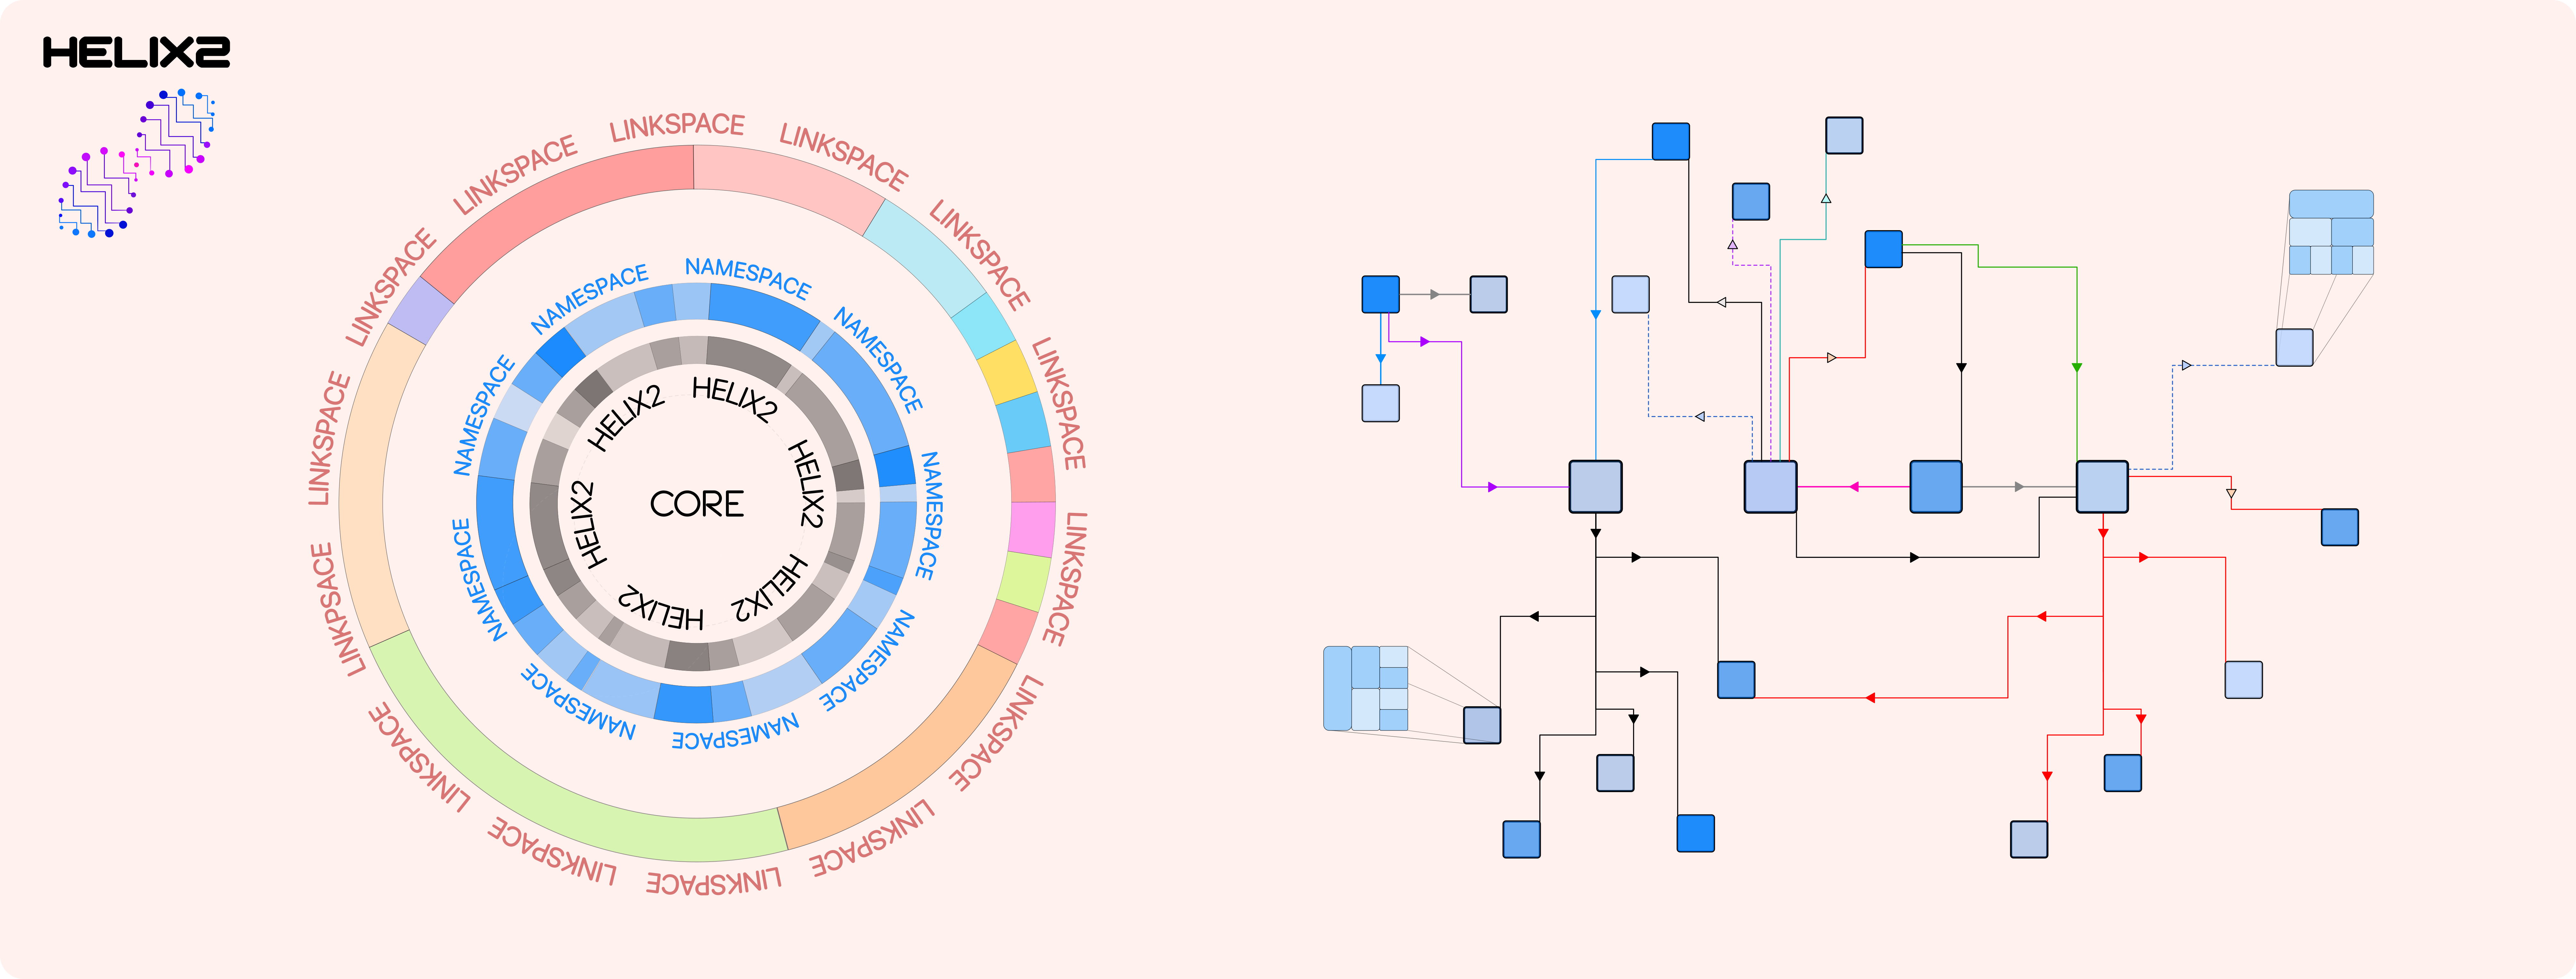
\includegraphics[width=160mm]{../schema/gif/helix2-schema_2.png}
\end{figure}
\begin{flushleft}
\textls[-50]{\mono{\href{https://helix2.xyz}{Helix2} is designed as a next-generation successor of these name services. While the set of nodes form a canonical and natural choice for labeling in any distributed system (e.g. addresses on any blockchain), the observation nonetheless is that most nodes do not interact with each other. For instance, there are about 220 million Ethereum addresses whereas an average address will likely interact with no more than a few hundred other addresses its lifetime. This means that most wallets have a limited set of interactions with contracts and addresses in general and their interactions are classifiable to a very large degree. Keeping this in mind, Helix2 is an attempt to provide Ethereum with a next-generation link service, in addition to the name service already provided by ENS. The expected outcome of the Helix2 protocol is a link-native naming ecosystem, a 'linkspace', where an interaction between two names is representable on-chain similar, but not limited to, a human-readable name for an address. A shift in focus from nodes to links has a profound effect on the nature of structures that an ecosystem can support. Several features which are challenging to achieve with a name service alone become extremely convenient with Helix2. For instance, Helix2 comes with several fundamental and easily accessible structural features such as stealth payments, social graphs, DAOs etc.\\
\vspace{0.2in}
While Helix2 has its own namespace, it does not replace ENS and is in fact intended to work alongside ENS as an extension. Helix2 is able to import all \tcbox{\mono{.}} namespaces by design without any bridging or wrapping. Lastly, Helix2 is not the only link service in the works; \href{https://woolball.xyz}{Woolball} is another link service currently under development although the two implementations arguably have more differences than similarities.}}
\end{flushleft}
\begin{flushleft}
\textls[-50]{\mono{

}}
\end{flushleft}
\begin{multicols}{2}
\bibliographystyle{plainnat}
\bibliography{}
\end{multicols}
\end{document}